\chapter{Supplementary Material}
\centerline{\rule{149mm}{.02in}}
\vspace{2cm}

TODO: intro to section

\begin{landscape}

	\null  % Empty line
	\nointerlineskip  % No skip for prev line
	\vfill
	\let\snewpage \newpage
	\let\newpage \relax
		\begin{figure}[H]
			\centering
			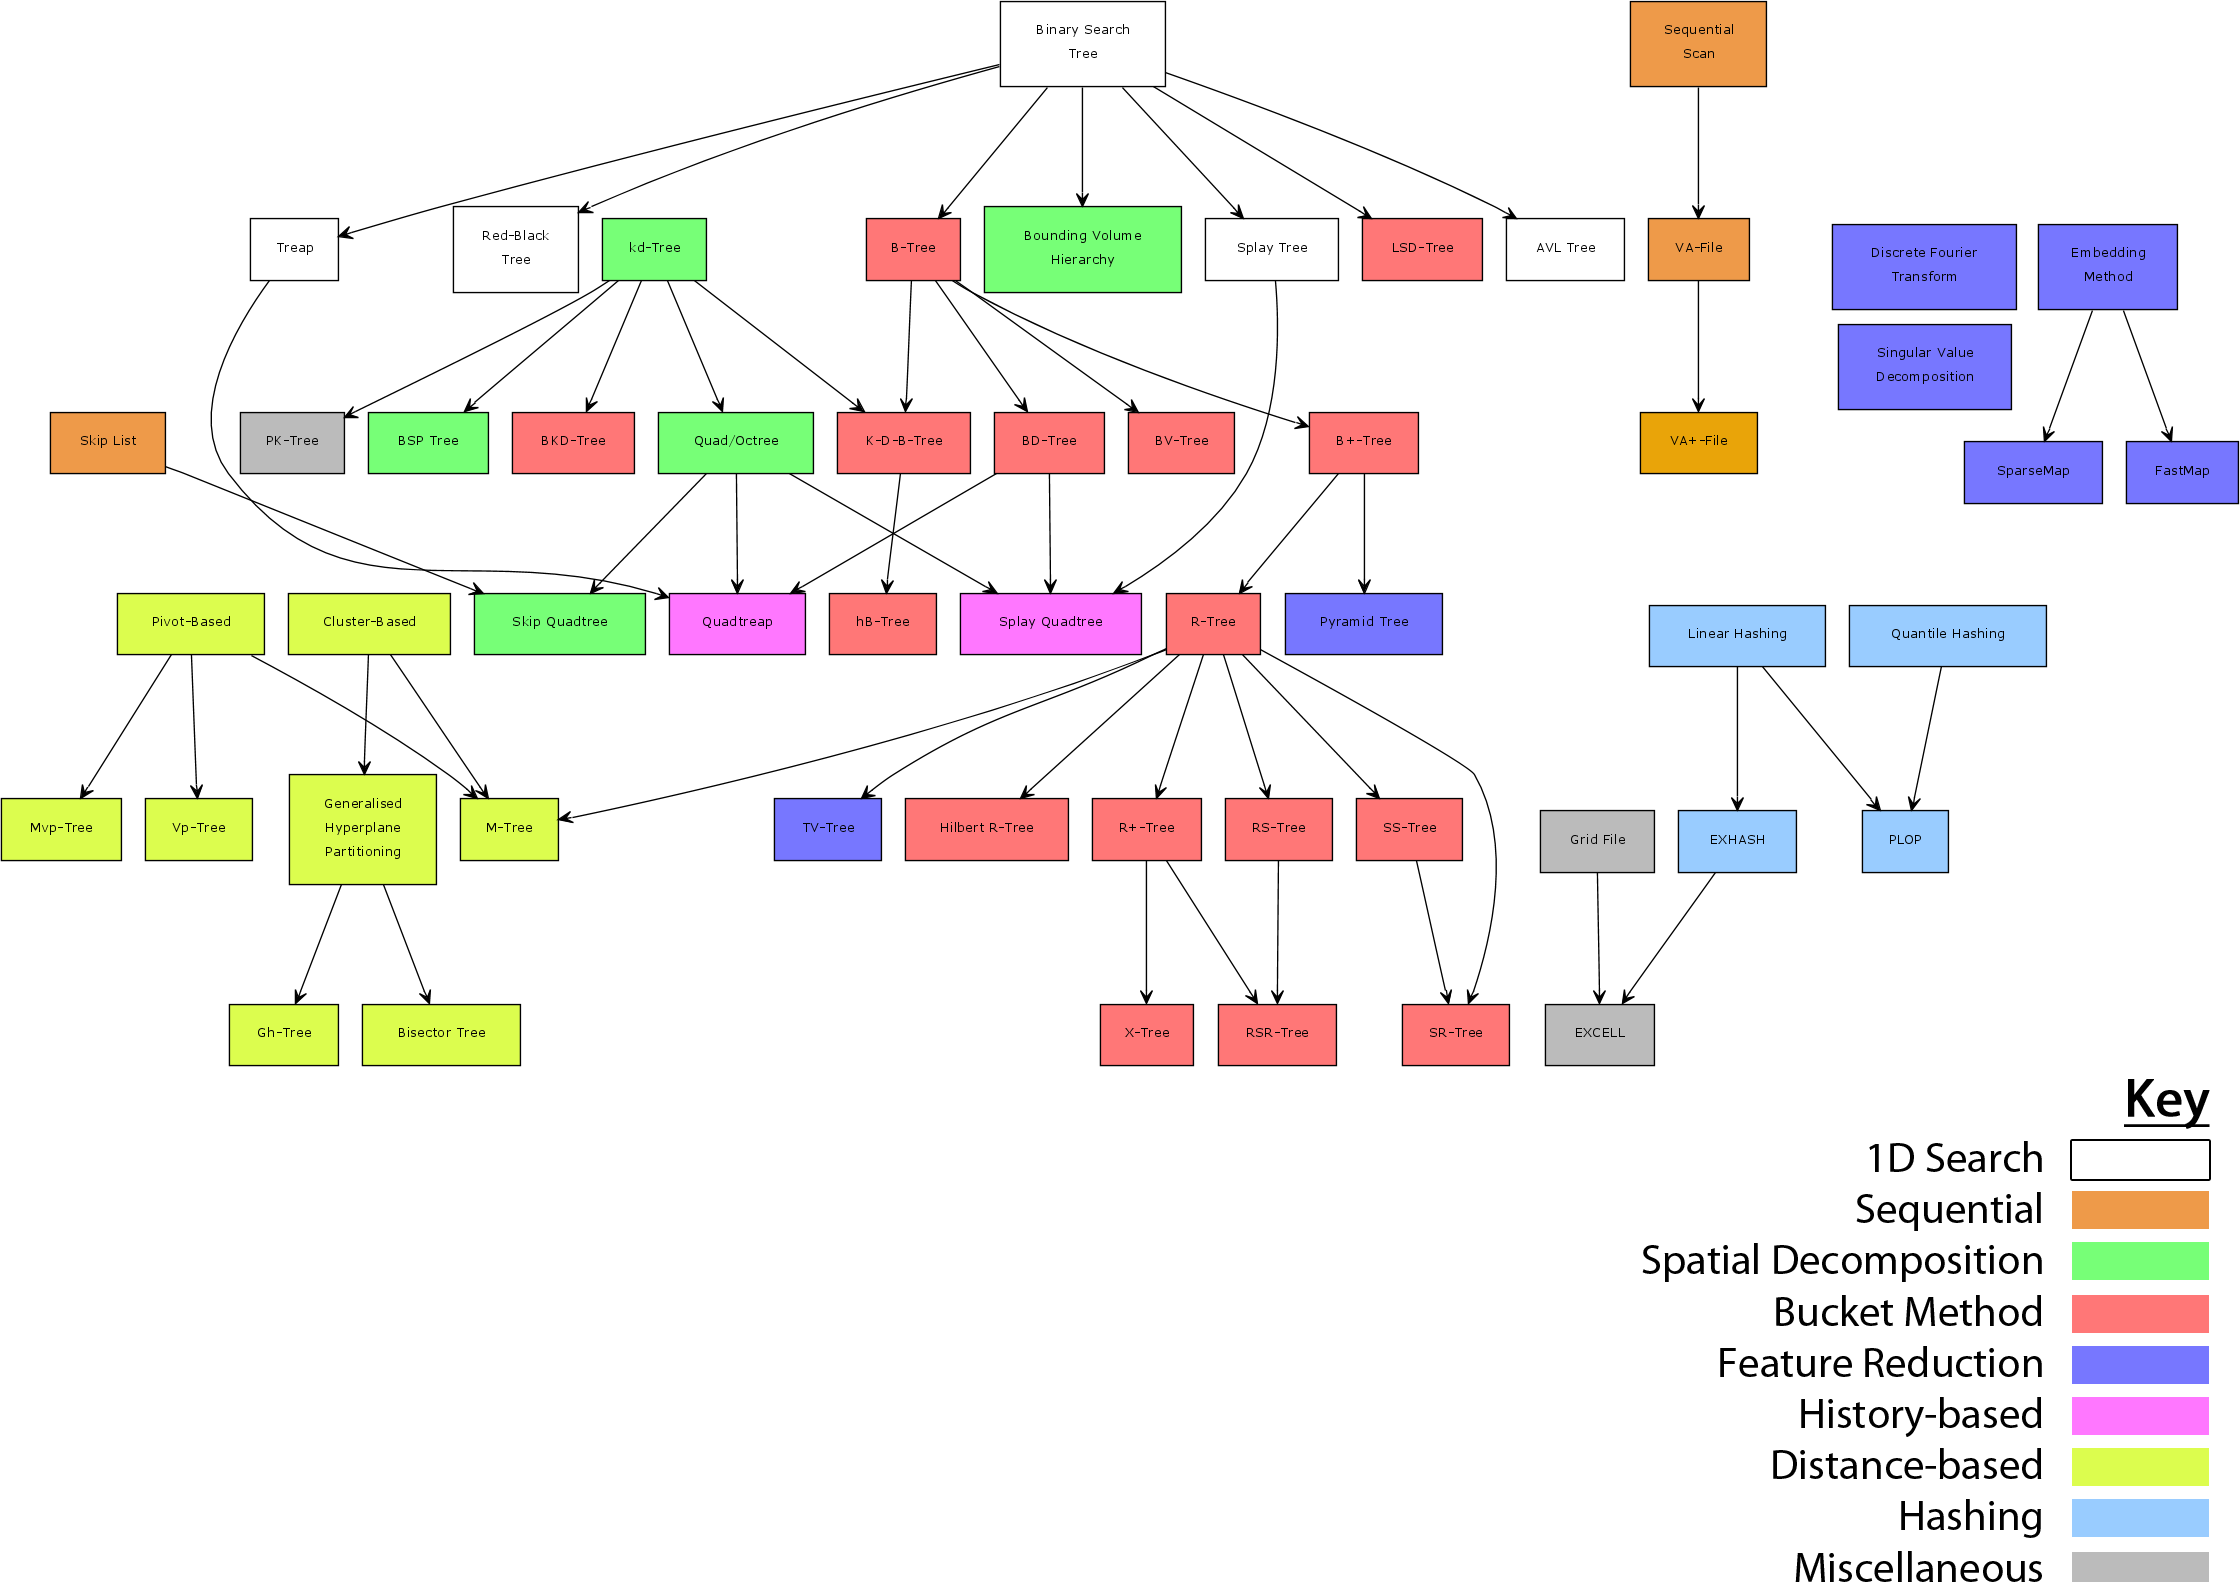
\includegraphics[scale=0.35]{figures/md_structure_taxonomy.png}
			\caption{Multi-dimensional Search Structure Taxonomy}
			\label{fig:structure-taxonomy}
		\end{figure}
	\let \newpage \snewpage
	\vfill 
	\break % page break

	\newpage

	\begin{table}
		\centering
		\begin{tabular}{|p{2.8cm}|p{5cm}|p{5cm}|p{5cm}|p{2cm}|}
			\hline
			\textbf{Index Structure} &
			\textbf{Memory Overhead} &
			\textbf{Bucket Method?} &
			\textbf{High-Dimensional Data} &
			\textbf{Complexity} \\
			\hline
			Sequential Scan & Low & No (but since data is stored contiguously, there are minimal I/O operations due to sequential access) & Often better than other structures with high $d$ (but significantly poorer performance with low $d$) & Low \\		
			B${}^{+}$-Tree & Low & Yes & One-dimensional & Low \\
			R-Tree & Moderate & Yes & Poor for $d > 10$ \cite{pyramid-tree} & Moderate \\
			Quadtree & Low with uniformly distributed data, high for skewed data due to unnecessary nodes caused by splitting sparse regions of data space & No & Poor because it tries to use balanced splits \cite{pyramid-tree} & Low \\
			Pyramid Tree & Low & Yes (based on B${}^{+}$-tree) & Good & High \\
			PK-Tree & Moderate & No (but uses similar method to reduce I/O operations) & Good & High \\
			Skip Quadtree & Moderate & No & Untested & Moderate \\
			Quadtreap & Low & No & Untested & Moderate \\
			Splay Quadtree & Moderate & No & Untested & Moderate \\
			\hline
		\end{tabular}
		\caption{Comparison of Dynamic Multi-Dimensional Structures}
		\label{tab:comparison}
	\end{table}

\end{landscape}